
\documentclass[a4paper,12pt]{article}
\usepackage[basque]{babel}%eee
\usepackage{fullpage}%margina
\usepackage{graphicx}%irudiak erabili 
\usepackage{amsmath}%matrizeak erabili, taulak
\usepackage{listings}%Kode zatiak txertatu

\lstset{
%    language=Java,
%    Letrak... aldatzeko kodean adibidez {->}{{$\rightarrow$}}1, aukera ezberdinak espazio batekin banatzen dira
%    literate=
    tabsize=4,
    numbers=left,
    stepnumber=1,             % the step between two line-numbers. If it is 1 each line will be numbered
    numbersep=5pt,            % how far the line-numbers are from the code
    frame=single,
%    sensitive=true,
    morecomment=[l][\color{darkgreen}\small\ttfamily]{//},
    morecomment=[s][\color{blue}\small\ttfamily]{/*}{*/}, %Eztakitx ondo dauen
    morestring=[b]",
    stringstyle=\color{red},
%    showstringspaces=false,
    numberstyle=\small,
    numberblanklines=true,
%    showspaces=false,
    breaklines=true,
%    showtabs=false,
    keywordstyle=\color{blue}\textbf
}

\usepackage[pdftex=true,colorlinks=true,linkcolor=blue,citecolor=black,urlcolor=blue]{hyperref}
\pagestyle{plain}

\makeatletter%Irudien kokapena beti htbp izatea gura dugu
 \def\fps@figure{htbp}
\makeatother

\usepackage[font=small,labelfont=bf,textfont=sl,justification=centerlast,labelformat=parens]{caption}

\begin{document}

% Aurkibidea berrizendatu
\renewcommand{\contentsname}{Aurkibidea}
% Bibliografia berrizendatu
\renewcommand{\abstractname}{Laburpena}
% Irudiak zenbaki arabiarrez
\renewcommand{\thefigure}{\arabic{figure}}

% irudi guztiak htbp lerrokapena izatea nahi dugu
\makeatletter
 \def\fps@figure{htbp}
\makeatother

\title{\textbf{IKT aktiboen eta IT zerbitzuen auditoria eta laguntzaren web-ingurune seguru baterako migrazioa}}
\author{Mikel Iturbe \\ Ibai Osa \\ Unai Pagalday}%+talde zenbakia
\date{}

\maketitle
\begin{center}
\bigskip
 
\includegraphics[scale=0.20]{irudiak/mgeplogo2.png}
\bigskip

 \today{}a
\end{center}



\thispagestyle{empty} %numeraziorik ez azalean % azala

\newpage

\vspace*{\fill}
\begin{abstract}
\noindent Lan monografiko honetan, ITILeko praktika onei jarraiki inzidentziak (enpresako IT zerbitzuetan jazotako edozein anomalia) jakinarazteko zerbitzu seguruaren inplantazioa jorratzen da. Horretarako, prozesu osoaren deskribapena egiten da: ITIL prozesuak lokalizatzea, garapena, segurtasun azpiegituraren (firewall, VPN) eraikitzea... Atal kronologiko desberdinetan jarrita: arazoaren hasieratik hasita, bukaerako ondorioetara arte. Era berean, diseinu eta garapen ahalik eta eraginkorrena izateko, ondo aztertuko dira software ingeniaritzak eskaintzen dituen metodologia desberdinak. 
\end{abstract}

\vspace*{\fill}

\newpage

\tableofcontents % Aurkibidea


\listoffigures%Irudien zerrenda

\section*{Introduction}
\addcontentsline{toc}{section}{Sarrera}

A P2P program, essentially, is an application that is used to share content through the network. Its most important difference from other downloading methods (FTP servers etc.) is that there is no central node in which content is downloaded from and uploaded to. The content flows through a decentralized network of nodes, clients, who simultaneously work as servers (or seeders, because they seed content) and downloaders (leechers). The most famous of them is eMule or aMule (depending on the Operating system used).

To illustrate different steps in the development phase, different kinds of diagrams have been used, starting from the user case diagrams in the very beginning until the fully-detailed class-diagram, all of them constructed using UML (the Unified Modelling Language). To make possible having different ends working at the same time, the resulting application is a distributed one, built using a Corba (Common Object Request Broker Architecture) implementation in the Java language, JacORB.


\begin{flushright}
The authors, Arrasaten, in Arrasate the \date{\today}.
\end{flushright}
 %sarrera

\section{Methodology}
\label{sec:met}

Being the already cited problem the creation of a P2P (Peer to Peer) application, it is vital to first identify the aspects that a P2P program normally fulfills, in order to work correctly. A P2P program, essentially, is an application that is used to share content through the network. Its most important difference from other downloading methods (FTP servers etc.) is that there is no central node in which content is downloaded from and uploaded to. The content flows through a decentralized network of nodes, clients, who simultaneously work as servers (or seeders, because they seed content) and downloaders (leechers). They are also servers in the P2P network, but they have a different role:
 
\begin{description}
 \item [Servers] Servers are used to identify and contact different clients between them. They do not take part in the actual process of downloading or uploading content, that is the clients' job. If the server infrastructure falls down, it can be replaced with a new one; no data is lost.
 \item [Clients] The core relies on the clients. Those are the responsible for downloading and uploading content, all the heavy traffic is done between clients, the server only helps meeting clients with similar interests. Normally, clients can stop and resume processes, and hold different processes at the same time (both uploads and downloads). More advanced features consists of bandwidth usage and a virtual crediting system to give priority to clients who share most. 
\end{description}

Thus, if we leave the more advanced features aside, we have already defined what our program should do, with its two main parts: servers and clients. The server (a main one is enough to build a prototype) is the responsible to put clients together and clients are responsible for moving content. The client is the one an average user would use, so it is the one we will focus on. The server needs no user interaction.

%Casos de uso diagrama
\begin{figure}
   \centering
   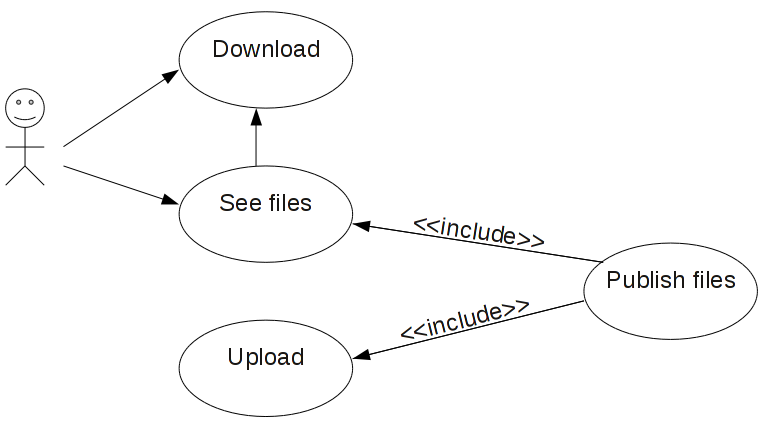
\includegraphics[scale=0.5]{irudiak/usercase.png}
   % Laster-markak gehitzeko menua
   \caption{User Case diagram of the P2P client}
   \label{fig:usercase}
\end{figure}

The diagram no. \ref{fig:usercase} shows the User Case diagram of the client, from the point of view of the user. When the user starts the program, receives from the server the list of the files available (the ones that other users have published) and chooses which one of the files wants to download. Without the user's consent, the files he or she is sharing are sent to other clients and if other clients want one of the files the user has, the upload of the content will also start automatically. Different uploading and downloading processes can be carried at the same time. 

It has to be mentioned though, that the user can control the content he or she wants to upload, but not through this application. All the content the user wishes to share is stored in a directory called \texttt{ongoing}, so the user can use the Operating System to put or remove different files in the directory, but as said, it cannot be done using the program. Likewise, all the downloaded content is stored in a directory called \texttt{incoming} and once the file is downloaded, it is the user who places the file in the directory he or she wishes to.

Before continuing with in-depth analysis and design of the application, it has to be cleared how many connections are there going to be. It has been noted before, that the main connections (the ones sharing content goes through) are between clients and that clients only turn to servers to know what files are being shared. Once the desired file has been selected and download starts from another client (or various, depending on the case) the server just keeps updating the downloadable file list, based on the clients that connect and disconnect. 

\begin{figure}
   \centering
   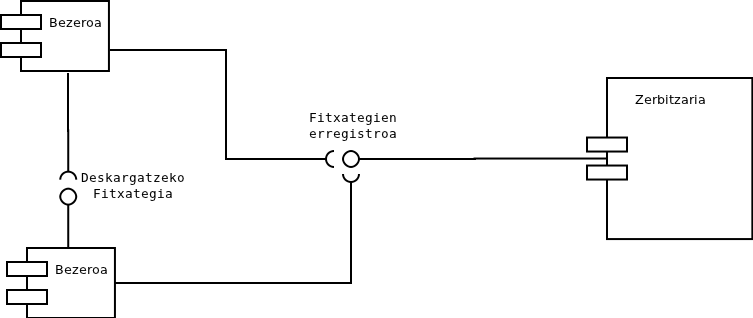
\includegraphics[scale=0.5]{irudiak/Loturak.png}
   % Laster-markak gehitzeko menua
   \caption{Connections in the P2P system}
   \label{fig:lotura}
\end{figure}

What has been told previously is summarized by the figure no. \ref{fig:lotura}. The diagram shows how the clients connect to the server to register files (and to receive the last version of the list showing the available files), and once they have selected what file to download, the server puts in contact the two clients (here the simplest case is shown, but more clients can be involved in the process), the seeder (the one who uploads) and the leecher (the one who downloads) start transferring content, but they still maintain contact with the server, to update the file list and to have the possibility to connect to other clients.

Finally, it is important to note that although general diagrams of the working programs have been done \textit{before} the application was developed, technically deeper diagrams that come later have been outlined \textit{after} the application was developed, in order to be as accurate as possible. For the sake of cleanness, and to ease things as much as possible to the reader, diagrams that were outlined in order to guide the development of the program have not been included in this report, as those diagrams have gone through numerous changes from the original version until the final one.

Thus, programming started early enough to make non-structural changes to the main design, but the main aspects of the program remained the same. The IDL file, for instance, was defined early in the analysis stage and luckily, there has been no need to change it all along the development phase:

\begin{lstlisting}[language=IDL]
module erabilgarriak{
	struct FileData{
		string name;
		long long size;
		string hash;
	};
	interface DownloadFile{
		typedef sequence<octet, 1048576> Part;
		FileData getFileData();
		long getPartCount();
		long getPart(in long numPart, inout Part part);
	};
	interface Server{
		typedef sequence<FileData> FileDataArray;
		typedef sequence<DownloadFile> DownloadFileArray;
		boolean register(in DownloadFile file);
		boolean deregister(in DownloadFile file);
		boolean getLista(inout FileDataArray files);
		boolean getFile(in FileData data, inout DownloadFileArray files);
	};
};
\end{lstlisting}
 
All the development has been done using VCS (Version Control System), to make development as easy as possible and to minimize possible version collisions. Parallel to the development, documentation has also been done step by step, using VCS as well, taking advantadge of the capabilities of \LaTeX{} to be used in one of those systems. In the next section, all the application is explained, using different diagrams and screenshots. Even those are used to explain the correct functioning of the program, they can be seen as the next step in the unified process of the creation of the Peer to Peer program.

Until now, only the main lines of the program have been set. Once the main components and actions of the program are defined, it is necessary to jump to the next layer: what has been done, using the methods already mentioned, to achieve the program explained in the user case diagram (figure \ref{fig:usercase}).  %arazoaren analisia

\section{Diseinua}

\subsection{Informazio sistemak}
\label{sec:dinf}
\subsubsection{ITIL prozesuak}
Inzidentziak nola jasoko diren definitu aurretik, beharrezkoa da definitzea enpresak berak nola jokatuko duen inzidentzia bat jasotzerakoan, hortik gero plano praktikora jaitsi eta aplikazioa nola garatuko den pentsatuz. Baina, hori egin baino lehen, nahitaezkoa da IT departamentuaren egitura definitzea, hau da, departamentua nortzuk osatuko duten. Osaketa hori egiteko, 14 pertsona eskuragarri izango ditugula uste da.

Jarraian zerrendaturiko dira IT departamentuak kudeatu beharko lituzkeen zerbitzuak, heziketa arloko enpresa bat dela suposatuz:

\begin{itemize}
 \item Moodle
 \item Webgunea
 \item Web zerbitzuak (idazkaritza birtuala, intranet)
 \item E-posta zerbitzuak
 \item Erabiltzaileen kudeaketa
 \item Baliabideen kontrola (nominak, ERP-a)
 \item Datu-base desberdinen kudeaketa
 \item Sarearen kudeaketa (barne-sarea, interneterako sarbidea)
 \item Ordenagailu pertsonalen kudeaketa (instalazioak e.a.)
 \item Datuen segurtasuna kudeatu
\end{itemize}

Ikusita zerbitzuak zeintzuk diren, ikusi beharko da, gure bezeroei (enpresako gainerako zatia) eskaintzen diegun zerbitzu hauen arabera, nola egongo den banatuta gure departamentua, zerbitzu hauen garrantziaren eta eskatutako lanaren arabera. Era berean, departamentuaren muina da erabiltzaileen eskariak aztertu eta konpontzea, baita funtzionalitate berriak ahal den heinean txertatzea, enpresaren eguneroko jarduna ahalik eta gutxien oztopatu eta kontrara, berau bultzatzeko.

\ref{fig:egitura} irudian agertzen den moduan banatu dugu gure balizko departamentua:

\begin{figure}
\centering
   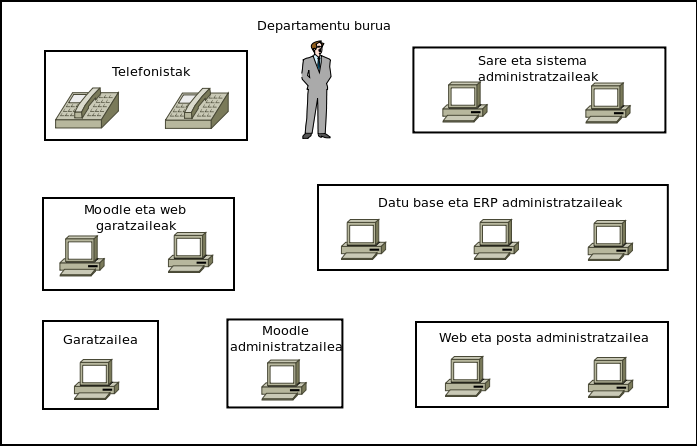
\includegraphics[scale=0.5]{irudiak/cau.png}
   % Laster-markak gehitzeko menua
   \caption{IT departamentuaren egitura}
   \label{fig:egitura}
\end{figure}


\begin{description}
 \item [Departamentu-burua] (pertsona bat). Izenak dioen moduan, gure IT departamentua eta beraz, Service Desk-aren burua izango litzatekeen pertsona da, formazio tekniko zein kudeaketarakoa duen pertsona litzateke berau, erabaki estrategikoak hartu eta azken hitza esateko ahalmena izateko. Era berean, gure departamentua eta gainerakoen arteko zubia litzateke, enpresako erabakietan informazio teknologien esparruan aholkatuz, edota soluzio berriak eskainiz. Ez luke parte hartuko zerbitzuen kudeaketa zuzenean, baina zerbitzuen araberako baliabideak lortzeko gaitasuna luke eta departamentuaren martxa on edo txarraren arduradun edo erantzule izango litzateke.

 \item [Hartzaileak] Bi pertsona. Arduraduna maila administratibo batean enpresarekin dugun lotura den bezala, hartzaileak, egunerokotasunean gertatzen diren gora-beheretzako kontaktuak lirateke. Zubia lirateke, beraz, gora-behera duten pertsonen eta gora-behera hori konpontzeko gai diren pertsonen artean. Arazoa konpontzeko erraza baldin bada edota askotan errepikatutakoa, eurak izango lirateke zuzenean erabiltzaileari eskaera konponduko lioketenak. Beraiek ikusiko lukete ea inzidentzia berriak dauden edo ez.

\item [Moodle eta Web garatzaileak] bi lirateke eta euren lana, Moodle-i funtzionalitate berriak gehitu edota web aplikazioak garatzea/eguneratzea litzateke, esate baterako, enpresako intranet sarean jartzeko.

\item [Garatzaile bat] Honek ere, aurrekoek bezala, aplikazioak garatuko lituzke, baina ez web ingurune baterako, baizik eta datu-base bateko interfazea, kalkuluak egiteko zenbait aplikazio... garatuko lituzke.

\item [Moodle administratzailea] Moodle zerbitzua behar bezala dabilela ziurtatuko duen pertsona da, erabiltzaileak alta eta baja emateaz gain. Bera litzateke arduraduna zerbitzua, gero ezarriko diren baldintzen pean mantentzeko.  

\item [Bi Web eta posta administratzaile] Hauek, webguneak, garaturiko web aplikazioak eta posta zerbitzua mantenduko luketen pertsonak dira, erabiltzaileentzat ahalik eta eskuragarrien jarriaz.

\item [Bi Sistema eta sare administratzaile] Sistema (zerbitzariak, erabiltzaileen ekipoak...) eta sarea kudeatuko luketen pertsonak dira.

\item [Hiru datu-base eta ERP administratzaile] Horietatik bi arduratuko lirateke ERPa kudeatzeaz eta bestea datu-baseko administratzaile modura. ERPko administratzaileetariko bat, datu-baseko administratzaile ere izan daiteke, besteari lagundu eta zerbitzu hobe bat eman ahal izateko.
\end{description}

Behin departamentua osaturik, bi hartzaile eta hainbat adituk osatuko luketela ikusirik, inzidentzia baten aurrean nola jokatuko litzatekeen definitu behar da, ITIL liburuetan azaltzen den modura. Gurean, \ref{fig:inzidentzia}. irudian ikus daiteke nola jokatuko den inzidentzia baten aurrean. Bertan,\textit{Arazoen kudeaketa} izeneko hitzak agertzen dira, baina hori askoz ere hedadura handiagoa duen gaia da eta lan honetako zioa baino askoz harago doa. Lan honetan suposatuko da, inzidentzia guztiak atoan konpondu edo bestela workaround (momentuko konponketa), zerbitzuaren aldaketa sakonak beste era batera landu beharreko gaia litzateke.

\begin{figure}
   \centering
   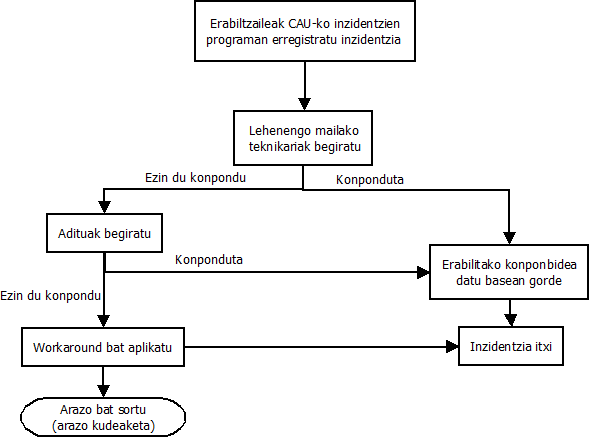
\includegraphics[scale=0.4]{irudiak/gestionInzidentzia.png}
   % Laster-markak gehitzeko menua
   \caption{Inzidentzien kudeaketa}
   \label{fig:inzidentzia}
\end{figure}

\subsubsection{CMDB}
Behin enpresan nola jokatuko den definiturik dagoela, behar-beharrezkoa da dokumentaturik izatea zeintzuk diren inzidentziekin loturik egongo diren elementuak, hau da, enpresako IT aktiboak. Beharrezkoa da ondo gordeta izatea aktibo bakoitza zer den, zein atributu dituen eta zein den aktibo horren jabe edo arduradua. Horretarako tresna, CMDB-a da.

CMDB (\textit{Configuration management database, Konfigurazioaren kudeaketarako datu-basea}) delakoa da inzidentziak gordetzeko web aplikazioaren muina. Bertan daude gordeta, IT teknologiekin loturiko enpresako aktibo guztiak (CI edo konfigurazio item-ak deritzena). \ref{fig:cmdb}. irudian ikus daiteke zein den CMDB-aren egitura. Aktibo gehienak taula berean daude jarrita, kodeak esleitzerako orduan erraztasuna izateko. Era berean, asmo horrekin garaturiko funtzioen bitartez sartuko dira datuak datu-basean, erabiltzailearentzat taulako NULL balio guztiak guztiz gardenak izango direlarik.

\begin{figure}
\centering
   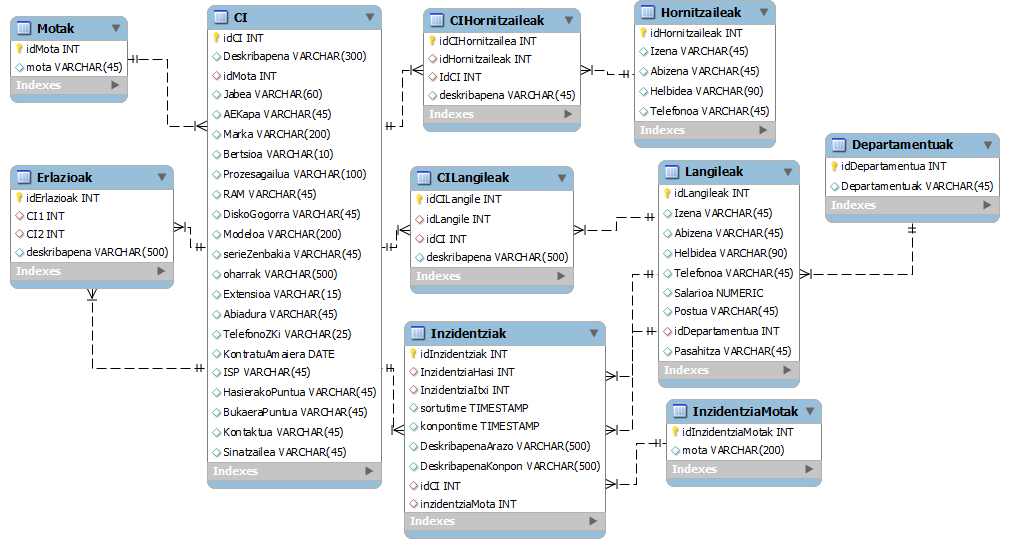
\includegraphics[scale=0.4]{irudiak/cmdb.png}
   % Laster-markak gehitzeko menua
   \caption{CMDB-aren eredu erlazionala}
   \label{fig:cmdb}
\end{figure}

\ref{fig:cmdb}. irudian ikus daitekeenez, inzidentziak gordetzerako orduan, inzidentzia kodea, inzidentzia zabaldu duen langilearen kodea, inzidentzia itxi duen langilearen kodea, inzidentzia hasi zen momentua, bukatutako momentua, inzidentziaren deskribapen laburra, konponketaren inzidentzia laburra, inplikaturiko konfigurazio itemaren kodea eta, azkenik, zein inzidentzia mota litzatekeen, motak, beste taula batean egongo lirateke, kategorizatuta. Era honetan, inzidentziaren inguruko datu guztiak gorde ahal izango lirateke, bertan.

\subsubsection{Inzidentzien web aplikazioa}
\label{sec:webapdis}
Erabiltzaileak web orrira sartzean izena eta pasahitza sartu beharko dute (datubasean hash baten bitartez egongo direlarik gordeta), gure enpresan lana egiten dutela ziurtatzeko. Behin sisteman logeatuta, inzidentziak sortzeko aukera, edo enpresako CI(configuration item) ezberdinak ikusteko aukera izango dute. Inzidentzia bat zabaltzerako orduan, langileek beraien kodea eta intzidentzia infektatzen dion itemaren kodea sartu beharko du, deskribapen batekin eta intzidentzia mota bat aukeratuz. 

IT departamentuko langileak badira ordea, honetaz gain jendeak zabalduriko intzidentziak ikusteko edota ixteko gaitasuna ere izango dute. Inzidentzia bat ixtean intzidentzia hori konpontzeko bete behar izan diren pausuak idatzi beharko ditu langileak, dokumentazio eta erreferentzia modura gordeta izateko.

\subsection{Metodologia}
\subsubsection{Kodifikazio manuala}
\ref{sec:webapdis} atalean azaldu den aplikazioa garatzen hasi baino lehen, beharrezkoa da jakitea aplikazioa \textit{nola} garatuko den. Ez funtzionalitate aldetik, horiek jada definiturik baitaude, baizik eta kode aldetik nola egongo den eginda. Era honetan lortzen dena da, kodearen estiloan uniformetasun bat bermatzea, egingo diren berrikuspenak erraztu (programatzaile bakoitzaren programazio-estiloak inpaktu txikiagoa izango baitu eta komentatuta egongo baita), bertsio berriak egitea errazteko (kodifikazio manualak, kodea berriztagarria izateko irizpideak lantzen baditu, bederen). Finean, kode eraginkorragoa eta ikuspegi profesionalagoa emango diona egitea dugu helburu. Irakurleak nahi izanez gero \ref{sec:kodman} eranskinean du ikusgai manuala osorik.

\subsubsection{Bertsio-kontrola}
Behin kodea nola idatziko dugun definitu dugula, beharrezkoa da era eraginkorrean kode hori garatzeko bitartekoak izatea. Hainbat pertsonen artean kodea garatuko delarik (era eraginkorrean espero da, horretarako sortu baita kodifikazio manuala), beharrezkoa da bakoitzak izango duen bertsioa azkena izatea, integraziorako aldaketak ez egoteko eta garatzaile guztiek funtzionalitate aldetik bertsiorik osoena izateko. 

Gainera, funtzionalitate oso interesgarriak eskaintzen dituzte.

\begin{itemize}
 \item Kudeatu beharreko kodearen biltegiratzea.
 \item Kodeari aldaketak egitea ahalbidetzea.
 \item Eginiko aldaketa guztiak erregistratzea.
\end{itemize}

Beraz, ez da izango beharrezkoa garatzaile guztiek kode osoa izatea euren laneko makinetan, errepositoriotik deskargatu, bertan landu (aldaketa partzialak, fitxategiak gehitu, kendu...) besterik ez baitu egin beharko.  Gainera, ikusi ahal izango da nork egin duen zein aldaketa.

Gure kasuan Git softwarea aukeratu dugu, web zerbitzu bati lotura egonik, beti eskuragarri dago (guk zerbitzari moduan erabiliko geunkeen ordenagailu jakin batean gorde behar izan gabe kodea, baliabideak aurreztuz). Gainera, funtzionalitate gehigarri gisa, bezeroa ere sartu ahalko litzateke web interfaze horretara bere lanaren nondik norakoak nola doazen ikusi ahal izateko (hala nahi izanez gero, noski). Ezingo luke edukirik igo web interfazetik, baina ikusi ahal izango luke berau. \ref{sec:gitinp} atalean azalduko da tresna hau nola erabiltzeari buruzko argibide praktikoak.

Direktorioen estrukturari dagokionez, hiru direktorio nagusi leudeke: bat garapen nagusirako eta beste bi albo lanetarako (datu-baseko datuak eta proiektuaren dokumentazioa). Kasu honetan, direktorio laguntzaileen kasuan, ez luke lagunduko bertsio-kontrola eginez, baizik eta sarean dagoen errepositorioa izanez, fitxategiak gordetzeko.

\subsubsection{Berrikuspenak eta Frogak}
Berrikuspen eta frogen helburua, kodea behin sorturik dagoela ahalik eta arazo gutxien dituela bermatzea da, bai \textit{bug}ak bilatuz zein funtzionalitateak betetzen dituela ikusiz. Berrikuspenen helburua garatzaile batek idatzitako kodea beste garatzaile edo kodea irakurtzeko gai den beste norbaitek, ea bug-ik sortu daitekeen edo egin beharreko funtzionalitateak betetzen dituen garatzaileak sortutako kodea. Gure kasuan, lan-talde txikia izanik, jende desberdinak egindako kodea guk ikus dezakegu, sistematikoki. Aurretik aipaturiko errepositorioan kodea izanda, erraztu egiten du kodea begiratzearen lana. 
 
Frogei dagokionez, bi eratako frogak daude, kutxa beltzekoak eta kutxa zurikoak. Kutxa beltzekoetan ez da kodea begiratzen eta aplikazioak ea espero den moduan jokatzen duen aztertzen da, hau da erabiltzaile normal batek, kode itxiko aplikaziobatean erreportatuko lukeena, gauza jakin bat ezin daitekeela egin aplikazioarekin. Kutxa beltzeko frogen helburua, erabiltzaileak egin ditzakeen pausuak errepikatzea da (funtzionalitateak eskura izanik), erroreak geronek ikusteko, erabiltzailearengana heldu baino lehen.

Kutxa zuriko frogak, jada kodea ikusgai daukagularik egiten dira (hortik izena, gardentasuna-edo erakutsiz) eta kodean dauden balioen arabera egiten dira frogak (String bateko balioak zeintzuk diren ikusirik, balio hori baino handiagoak jarriaz, adibidez edo funtzio bati beste aldagai mota bat pasaz). 

\noindent \textbf{Definituriko frogak}
\noindent \textbf{Kutxa beltzeko frogak}

\begin{itemize}
\item Erabiltzaile izen edo pasahitz oker bat sartu
\item Langile arrunt baten erabiltzaile izen eta pasahitz zuzenak sartu eta aktiboak ikusteko aukeratu
\item Informatikari bat logeatu eta inzidentzia historikoak ikusi
\item Informatikari bat logeatu eta inzidentziak ikusi
\item Informatikari batek inzidentzia berri bat sortu ondoren inzidentziak ikusteko sakatu-
\item Informatikari batek inzidentzia bat itxi eta inzidentziak ikusteko sakatu
\item Informatikari batek inzidentzia bat itxi eta inzidentzia historikoak ikusteko sakatu
\end{itemize}


\noindent \textbf{Kutxa zuriko frogak}
\begin{itemize}
\item Inzidentzia bat sortu eta begiratu inzidentzia berriarentzat kode berri bat sortzen den automatikoki
\item Inzidentzia bat sortu eta begiratu inzidentzia hori sortu den data benetan sortu den dataren berdina den.
\item Inzidentzia bat sortu erabiltzaile batekin eta begiratu ea inzidentzia sortu duen erabiltzailearen kodea benetan inzidentzia sortu duenarena den.
\item Inzidentzia mota berri bat sartu datu basean eta begiratu ea inzidentzia mota berri hori comboboxean agertzen den
\item Aktibo berri bat sartu eta ondoren begiratu aktibo hori agertzen dela.
\item Inzidentzia bat itxi eta begiratu konponduta parametroaren egoera aldatzen den.
\item Inzidentzia bat itxi eta begiratu inzidentzia itxi duen langilearen kodea ongi gordetzen den.
\item Inzidentzia bat itxi eta begiratu inzidentzia itxi den data ongi gordetzen den.
\end{itemize}

\subsection{Segurtasuna}
\label{sec:dsec}
Aipatu bezala, beraz, web aplikazioa sare lokaletik kanpo joango da, baina era berean kanpoko saretik babestuta joango den inguru batean. Inguru horri, DMZ (\textit{DeMilitarized Zone,  zona desmilitarizatua}) deritzo, bi \textit{fronte} ezberdinen arteko mugan baitago, aparteko ingurune batean. Era honetan, bertara sarbidea kontrolatuko duen firewall-aren bitartez, sare lokaletik eta kanpotik, VPN bat erabilita sartu ahal izango da.

\begin{figure}
\centering
   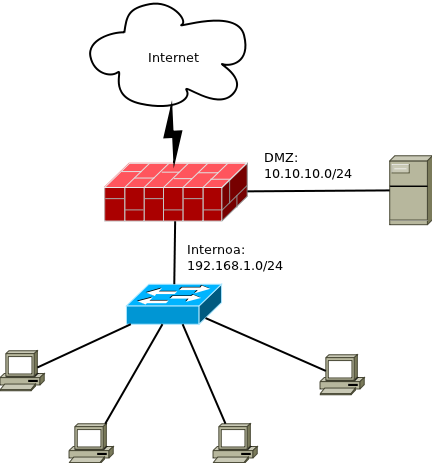
\includegraphics[scale=0.5]{irudiak/sarea.png}
   % Laster-markak gehitzeko menua
   \caption{Sarearen eskema}
   \label{fig:sarea}
\end{figure}

Firewall-ak, horretarako, konexioak baimendu behar ditu, bai sare lokal eta DMZ artean, baita kanpotik datorren VPN bitartezko trafikoa (kanpoko langileak eta batez ere zerbitzu teknikoko enpresa) ere. Beste konexio guztiak deseginez, DMZ horren segurtasuna bermatzen dugu, guk espreski baimentzen ez diogunari sarbidea ukatuz.

Laburbilduz, hauek lirateke Firewall-eko oinarrizko arauak (portuak ez dira esplizituki adierazi, zerbitzu bakarra dagoelako, suposatuko da, zerbitzaria helburu duten paketeak 80. portura joango direla eta erantzunak $>1024$ portuetara).
\bigskip


\begin{tabular}{|c|c|c|c|c|c|}
\hline
 Jatorrizko helbidea & Helburu helbidea & Protokoloa & Flag-ak & Ekintza \\ \hline
 192.168.1.0/24 & 10.10.10.0/24 & http &  & Baimendu \\ \hline 
 10.10.10/24 & 192.168.1.0/24 & http & STB & Baimendu \\ \hline
 192.168.1.0/24 & ANY & http &  & Baimendu \\ \hline
 ANY & 192.168.1.0/24 & http & STB & Baimendu \\ \hline
 220.100.65.98 & 10.10.10/24 & vpn & & Baimendu \\ \hline
 10.10.10/24 & 220.100.65.98 & vpn & STB & Baimendu \\ \hline
 ANY & ANY & ANY & & Ez baimendu \\ \hline
\end{tabular}

Era honetan, zerbitzu teknikoko enpresakoek (zeina 220.100.65.98 helbidea erabiliko luketen), gure enpresakoekin batera kontsultak egin ahal izango lukete sarearen bitartezko VPN trafiko zifratua erabiliz. VPN zerbitzaria, Firewall-eko 10.10.10/24 sareko gateway-ean egongo litzateke eta beste enpresakoak, bertako IP helbidea jakinda, euren VPN bezeroa erabiliz konektatu ahalko lirateke, baina, esan bezala, bakarrik euren enpresako helbidetik. %soluzioaren diseinua

%problems with one MB (goes but performance goes down a bit)

\section{Inplementazioa}
\subsection{Informazio sistemak}
Web aplikazioa, JSP (\textit{JavaServer Pages}) erabilita sortu da, azpitik Java erabiliz. Honen arrazoi nagusia, webgune dinamikoak sortzeko duen erraztasuna, datu-basearekin konektatzeko eginiko funtzioak eta duen integrazio maila altua da.

Txosten honen helburua berau ez denez, labur-labur azalduko da webgunearen egitura: 

Web orrira index.jsp orritik sartzen da, behin logeatuta beste orrietara sartzeko baimena izango duelarik erabiltzaileak: inzidentziak.jsp inzidentziak ikusteko, inzidentziaSortu.jsp inzidentziak sortzeko eta aktiboakIkusi.jsp aktiboak ikusi ahal izateko. Web orriak akzio bat egitean kontrol.jsp-ra doa, honek egin beharreko kalkuluak egin ostean behar den orrira berbideratzen du, aktiboakIkusi.jsp orrian izan ezik, horri honetan comboBox bat egongo da aktibo mota aukeratu ahal izateko, comboBox honen submit-a fitxategia beraren aurka egingo da. Beste bi fitxategi ere badaude  aktiboakTaula.jsp eta inzidentziaTaula.jsp bi orri hauek iframe-en bidez sartuko dira beste web-orrietan, taulak bistaratzeko bakarrik dira.

\subsection{Metodologia}
\subsubsection{Bertsio kontrola}
\label{sec:gitinp}
Aurreko diseinu atalean aztertuz gero zein erraminta erabiliko den eta zergatik, oraingoan Git (Github errepositorio zentral modura) nola konfiguratu eta erabili. IDE batekin sinkronizatu beharrean, zuzeneko metodoa erabili da, komando-lerroa erabiliz. Git instalatu ondoren, gure proiekturako konfiguratu behar da, erabiltzailearen izena eta e-posta helbidea jarriaz:

\begin{verbatim}
git config --global user.name "popbl6"
git config --global user.email popbl6@gmail.com
\end{verbatim}   

Behin konfiguraturik, has gaitezke lanean:

\begin{verbatim}
mkdir POPBL6                                            (proiektuaren direktorioa 
                                                        sortu)

cd POPBL6                                               (direktoriora joan)

git init                                                (git errepositorio 
                                                        hutsa sortu)

touch README                                            (READMEa sortu)

git add README                                          (fitxategia indizera 
                                                        gehitu)

git commit -m 'lehen commita'                           (aldaketa egin 
                                                        errepositoriora, 
                                                        lehen commita mezuarekin)

git remote add origin git@github.com:popbl6/POPBL6.git  (Github-en dagoen 
                                                        errepositorioa gehitu
                                                        origin izenarekin)

git push -u origin master                               (gure errepositorio 
                                                        lokaleko adar nagusia  
                                                        Github-era pasa)
\end{verbatim}

Github-eko azken kodea hartzeko, aldiz, nahikoa da gure errepositoriora joan eta hau idaztea:

\begin{verbatim}
git pull origin
\end{verbatim}

Automatikoki hartuko du bertako adar nagusia (\textit{master} defektuz). Agindu honek bi ekintza egiten ditu: lehenik eta behin norberaren errepositorioan ez dauden commit-ak (ekarpen kodean) jaitsi (\texttt{fetch} ekintza) eta gero, jaitsitakoa eta errepositorio lokala batu (\texttt{merge} deritzona). Era honetan, sinkronizaturik geratuko dira guk lan egiteko erabiltzen dugun errepositorio lokala eta github-eko zentrala.

\subsection{Segurtasuna}
Atal honetan, azalduko dena da nola konfiguratu den erabili den Fortigate firewall-a Diseinu atalean planteaturiko soluzioa lortzeko. Dena dela, irakurleak interesa izanez gero, \textit{backup}eko konfigurazio fitxategi osoa aurkitu dezake \ref{sec:forkonf} eranskinean. Era berean, hainbat gauza gehigarri jarri dira (web filtroa e.a.), baina ez denez txosten honetako muina, ez dira jorratuko hemen.

Lehenik eta behin, Firewall-aren interfazeak konfiguratu behar dira (gogoan izan behar da diseinuko atalean azaltzen den \ref{fig:sarea} irudia):

\begin{verbatim}
System > Network > Interface > dmz

Addressing mode               Manual
IP/Netmask                    10.10.10.1/255.255.255.0
Administrative access         PING
\end{verbatim}

Adibide moduan jarritako DMZko interfazeaz gain, beste biak (barne-sareari eta \texttt{wan1}, internetera konektatuko lukeen interfazeak) antzera konfiguratu behar dira. Behin hiru interfazeak konfiguraturik daudela, beharrezkoa da firewall-eko erregelak kargatzea:

\begin{verbatim}
Firewall > Policy

Source Interface / Zone           internal
Source Address                    FinEng
Destination Interface / Zone      wan1
Destination Address               All               
Schedule                          Always
Service                           ANY
Action                            ACCEPT
NAT                               Enable 
Protection Profile                standard_profile
\end{verbatim}

Erregela honekin, FinEng taldeari dagozkion helbideetatik (taldearen sorrera ez da jorratzen hemen, baina era berean, sare interno osoari dagokion helbidea jar daiteke bertan), edonora doazen konexioak baimentzen dira, \texttt{standard\_profile} profila aplikatzen zaielarik (guk sortua) eta NAT ere aktibatuz.

Era berean aplikatu daiteke DMZn egongo den zerbitzarira konektatzeko:

\begin{verbatim}
Firewall > Policy

Source Interface / Zone           internal
Source Address                    FinEng
Destination Interface / Zone      dmz
Destination Address               10.10.10.5               
Schedule                          Always
Service                           ANY
Action                            ACCEPT
NAT                               Enable 
Protection Profile                standard_profile
\end{verbatim}

Suposatuz, noski, zerbitzariaren IP helbidea hor agertzen den 10.10.10.5-a delarik. Behin erregela horiek definituta, beharrezkoa da VPNa aktibatzea eta ostean erregela batzuk gehiago definitzea, kanpoko enpresako kideak konektatu ahal izateko gure zerbitzarira. Lehenengo, helbideei izenak emango dizkiegu.

\begin{verbatim}
Firewall > Address > New

Address name          DMZ sarea
Type                  Subnet / IP Range
Subnet / IP Range     10.10.10.0
Interface             Any
\end{verbatim}

\begin{verbatim}
Firewall > Address > New

Address name          Enpresa teknikoa
Type                  Subnet / IP Range
Subnet / IP Range     64.230.254.50
Interface             Any
\end{verbatim}

Esan behar da, bigarren IP helbidea, simulatzeko asmoarekin esleitu zaiola, \texttt{wan1}-en sare berean egon beharko duelako, baina, benetan beste sare batean egongo litzateke eta beste IP helbide guztiz desberdina litzateke.

Helbideak definiturik izanda, hurrengo pausua, Fortigate-ko aldeko VPNa konfiguratu behar da.

Lehen fasea konfiguratzeko:

\begin{verbatim}
VPN > IPSEC > Auto Key (IKE) 

Create phase 1

Name                    Enpresa teknikoa
Remote Gateway          Static IP Address
IP address              64.230.254.50
Local interface         wan1
Mode                    main
Authentication Method   Preshared Key
Pre-shared key          pasahitza
Peer options            edozein
\end{verbatim}

Bigarren fasea konfiguratzeko:

\begin{verbatim}
VPN > IPSEC > Auto Key (IKE) 

Create phase 2

Name                  enpresa_tunel_1
Phase 1               Enpresa teknikoa

> Advanced

Jatorrizko helbidea:  64.230.254.50
Helbide helburua:     10.10.10.0
\end{verbatim}

Era honetan, lehen fasearen ostean, sortuko den tunela konfiguratzen da, jatorria beste enpresak duen bezeroan egongo litzatekeelarik eta gure DMZko interfazeko VPN zerbitzaria izango delarik konexioaren helburua. Tunelak eginda, beharrezkoa da, tunel horien arteko trafikoa ahalbidetuko duen firewall erregela berriak.

\begin{verbatim}
Firewall > Policy

Source Interface / Zone          dmz
Source Address                   DMZ sarea
Destination Interface / Zone     wan1
Destination Address              Enpresa teknikoa
Schedule                         Always
Service                          ANY
Action                           IPSEC
VPN Tunnel                       enpresa_tunel_1
Allow Inbound                    yes
Allow outbound                   yes
Inbound NAT                      yes
Outbound NAT                     no
Protection Profile               standard_profile
\end{verbatim}

Era honetan, firewall-ak baimenduko du, enpresa teknikoko eta gure DMZn dagoen sarearen arteko VPN trafiko zifratua. Firewall eta VPN zerbitzaria konfiguraturik daudela, beharrezkoa da VPN bezeroa (FortiClient, zerbitzu teknikoko enpresak izango lukeena) konfiguratzea.

\begin{verbatim}
VPN > Connections

Connection Name            konexioIzena
Configuration              Manual
Remote Gateway             64.230.120.8 (FortiGate-aren wan1 interfazea)
Remote Network             10.10.10.0  / 255.255.255.0 
Authentication method      Preshared key 
Preshared key              1. fasean jarritako pasahitza
\end{verbatim}

Behin jada konektaturik dagoela eta martxan jarrita, inolako arazo gabe ikusi ahal izango dugu inzidentzia zerbitzariaren edukia.




  %soluzioaren inplementazioa

\section{Conclusions and future improvements}
%optimizazioa hari globalak seederrak txekatzeko, deskargak bertan registratu eta guztiei eramateko erantzunak. eta gordetzailearekin berdin
%Deskargak gelditzea

The main conclusion draw is that modelling the IDL file correctly at the beginning, analysing the functionalities and structure of the program beforehand, is crucial to have good rhythm of work. Changing the IDL and thus, the main structure of the program after starting the development, has very negative consequences in the course of development. We started later developing, because of multiple changes in the IDL and design of the program. But, in the long run, we gained many hours.

As far as future improvements are concerned, we have outlined two: there is no functionality of pausing or removing current downloads and it would be very interesting to have them, as it is one of the functionalities most Peer to Peer programs have. It would also improve user experience, because once a download starts, the user has no power over it until it is finished.

The other main improvement has little to do with user experience. It is closely related to performance. Our program uses multiple threads that eventually can lead to heavy CPU usage. Reducing CPU use is a priority if we want to be possible to use the program along with others comfortably. One partial simple solution we propose is to use a single \texttt{SeedChecker} to all of the downloads, where \texttt{Deskargak} would register and the checker would go individually over them. The same could be done with \texttt{Gordetzaileak}. That way, ther would be no extra threads per download and we think performance should improve, at least to a noticeable level, once the download number grows.%Ondorioak

\section{Hobekuntzak}
Hobekuntza posibleen artean nabarmendu daitezke eginiko aplikazioaren alorrean, CMDB-aren diseinu hobea (horrenbeste eremu nulo izango ez lituzkeena) edota inzidentzietaz harago doan kudeaketa eredu osoaren inplementazioa, ITILek eskaintzen duen bibliografia eta lan-tresna mardulak profitatuz.

Era berean, segurtasunari dagokionez, Firewall-aren diseinu errealistagoa egin daiteke, DMZtan beste zerbitzari batzuk jarriaz eta bertara kanpoko sarbidea baimenduz (web eta posta zerbitzariak, akaso). Era berean, barne saretik kanporako trafiko osoa baimenduta dagoen aldetik (web filtroekin, egia da), agian hori findu beharko litzateke eta konexio mota batzuk ez baimendu, segurtasun neurriak zorrozteko. Datu-basean, \textit{hash} algoritmo indartsuago bat erabiltzea ere ondo legoke, pasahitzen krakeoa zailtzeko.

Azkenik, erabilitako metodologiarekin, alderik nabarmenena, Github erabiltzerakoan erabiltzaile bakarra ez erabiltzea da, baizik eta garatzaile bakoitzak bere izena edo izenordaina erabiltzea, jakiteko zehatz-mehatz nork egin duen zer. Oraingo metodoarekin, talde guztiak dauka erantzukizuna, eta ez da maila pertsonalera heltzen.
%Balizko hobekuntzak

\appendix
\section*{Appendices}
\addcontentsline{toc}{section}{Appendices}

\section{Design patterns}
In software engineering, a design pattern is a general, repeatable and language-independent solution to a commonly occurring problem in software design. They allow people to communicate more easily, because programmers can use well known names and software interactions, and to understand exchanged code better. They also speed up the development process by providing tested efficient solutions to common programming problems.

Design patterns are divided into different groups depending on their purpose, creational, structural or behavioral are only some of them.

\subsection*{Creational design patterns}

The design patterns on this category concentrate on the creation and initialization of different objects.
One of the most used design patterns falls into this category, the singleton. This pattern is used when an instance of an object has to be used through all the program. We use this pattern when interacting with the different elements of the ORB and the server via the Globalak class.
\begin{lstlisting}[language=java]
public class A {
    private static A a;
   
    private A(){
        init();
    }

    public static A getA(){
        if(a == null) A = new A();
        return a;
    }
}
\end{lstlisting}
In this pattern the only way to use the \lstinline{a} field is calling the  \lstinline{getA()} function, and the constructor and the field being \lstinline{private} ensures that there is only one instance of \lstinline{A}.

Different factories are also in this category.


\subsection*{Structural design patterns}

These patterns are about class and object composition and how they interact between them using interfaces to obtain new functionalities.

The java graphical user interface framework, Swing, uses these patterns to create and manage different elements.


\subsection*{Behavioral design patterns}

This category concentrates on the communication between different objects.

In this category is the iterator that lets us iterate on a list.


\subsection*{Concurrency design patterns}

The patterns on this category deal with multi-threaded programming problems.

The thread pool or the different kinds of using shared resources fall into this category

\section{Bibliography}

\noindent THE JACORB TEAM. \textit{JacORB 2.1 Programming Guide} [online]. The JacORB Team, 2004. \newline \htmladdnormallink{http://jmvanel.free.fr/corba/doc/jacorb-ProgrammingGuide.pdf}{http://jmvanel.free.fr/corba/doc/jacorb-ProgrammingGuide.pdf} [Last consultation: 6-13-2011]
\bigskip

\noindent GITHUB. \textit{GitHub:Help} [online]. GitHub, 2011. \newline \htmladdnormallink{http://help.github.com/}{http://help.github.com/} [Last consultation: 6-13-2011]
\bigskip

\noindent GAMMA, Erich; HELM, Richard; JOHNSON, Ralf; VLISSIDES, John M. \textit{Design Patterns: Elements of Reusable Object-Oriented Software}. Boston: Addison-Wesley Professional, 1994. \newline 
\bigskip




\end{document}